% CVPR 2025 Paper Template
\documentclass[10pt,twocolumn,letterpaper]{article}

% *** CVPR packages ***
\usepackage[pagenumbers]{cvpr}
\usepackage{graphicx}
\usepackage{amsmath}
\usepackage{amssymb}
\usepackage{booktabs}
\usepackage[breaklinks=true,bookmarks=false]{hyperref}
\usepackage{xcolor}
\usepackage{float}

\def\cvprPaperID{****}
\def\confName{EEE 515}
\def\confYear{2026}

\begin{document}

\title{EEE 515 --- Final Project Prep:\\Reading Assignment and Discussion Post}

\author{Ankur\\
EEE 515: Computer Vision --- Spring 2026\\
Arizona State University\\
{\tt\small ankur@asu.edu}
}

\maketitle

% ===================================================================
\section{Reflection on Research Experience}
% ===================================================================

The only time I have been exposed to research has been in my course projects as an undergraduate and graduate student and not as a thesis course and laboratory research. On such projects, I was guided by a systematic workflow, that is, identifying a problem, reviewing what is being available in the market, applying a technique, and assessing the outcomes, but I realize this is not how real research works, as it would require to come up with new questions and go beyond what is already available. This distinction became solid with the reading of William T.\ Freeman in his article about how to do research, titled, of course, exactly that, namely: ``\textit{How to do research}'' \cite{freeman}. Freeman points out that beginning with defining significant open problems, rather than rushing to solutions, is the hallmark of good research, and that reading widely and broadly within the literature is a crucial aspect of knowing where real gaps exist. Another key point that he offers, which I find life-affirming in the final project preparation, is the importance of perseverance, intellectual integrity, and learning by making mistakes.

Intriguingly, the experience of writing this assignment was a demonstration of the advice that Freeman provided. My original project proposal, which was a mixture of SplaTAM and LangSplat to create open-vocabulary SLAM, appeared to be unique until I conducted an intensive literature review and found that other separate teams had already published their systems. This experience revealed the importance of thorough literature review by Freeman that must be done prior to committing resources to a direction. Instead of being disheartening, I used this finding to determine a real gap---dynamic scene handling in language-embedded SLAM---which formed the foundation of a more powerful, more differentiated proposal.

% ===================================================================
\section{Paper Summary: From 3D Gaussian Splatting to Language-Embedded SLAM in Dynamic Worlds}
% ===================================================================

\subsection{Overview}

The field of 3D scene representation has evolved rapidly since the introduction of 3D Gaussian Splatting (3DGS) \cite{kerbl20233dgs}, which replaces implicit neural representations (e.g., NeRF) with explicit, differentiable 3D Gaussians enabling real-time rendering. Three parallel threads have emerged: (1) 3DGS-based SLAM systems for real-time mapping, (2) language-embedded Gaussians for open-vocabulary scene understanding, and (3) dynamic scene handling. Below, I summarize five key papers spanning 2023--2024 that inform my proposed project.

\subsection{Paper Summaries}

\textbf{1. 3D Gaussian Splatting for Real-Time Radiance Field Rendering} \cite{kerbl20233dgs}. This foundational work models scenes as collections of anisotropic 3D Gaussians, each parameterized by position, covariance, opacity, and spherical harmonic color coefficients. Its tile-based differentiable rasterizer achieves over 100\,FPS at 1080p---orders of magnitude faster than NeRF---while matching or exceeding visual quality. The explicit representation makes downstream extensions tractable: each Gaussian is an independent entity that can be augmented with semantic, language, or dynamic attributes without modifying the core rendering pipeline. The entire pipeline---initialization from Structure-from-Motion points, adaptive densification (splitting large Gaussians, cloning small ones), and pruning---is fully differentiable, allowing end-to-end optimization with photometric loss.

\textbf{2. SplaTAM: Splat, Track \& Map 3D Gaussians for Dense RGB-D SLAM} \cite{keetha2024splatam}. SplaTAM is the first system to use 3D Gaussians as the sole map representation for dense SLAM. It alternates between tracking (optimizing a 6-DOF camera pose by minimizing combined photometric L1 + SSIM and geometric depth L1 loss against the map via differentiable rendering) and mapping (optimizing Gaussian parameters and adding new Gaussians for unobserved regions). A silhouette-based expansion mechanism enables structured map growth. SplaTAM achieves $2\times$ improvement in tracking accuracy (ATE) over NICE-SLAM and Point-SLAM on the Replica dataset, with sub-centimeter ATE RMSE on most scenes and PSNR exceeding 30\,dB, establishing the viability of 3DGS for real-time robotic mapping. However, SplaTAM assumes a fully static environment and produces purely geometric maps with no semantic understanding.

\textbf{3. LangSplat: 3D Language Gaussian Splatting} \cite{qin2024langsplat}. LangSplat addresses the semantic gap by augmenting each 3D Gaussian with a language feature vector derived from CLIP. The key challenge is that CLIP features are high-dimensional (768-D for ViT-L/14), making per-Gaussian storage prohibitive for large scenes. LangSplat solves this through a scene-specific autoencoder that compresses CLIP features to a compact latent space (e.g., 16 dimensions) with minimal semantic loss. SAM (Segment Anything Model) generates multi-scale masks so that language features capture object-level rather than pixel-level semantics. At query time, a user provides a text prompt like ``find the chair,'' CLIP encodes it, and relevancy scores are computed against per-Gaussian language features to produce a 3D localization heatmap. LangSplat achieves $199\times$ speedup over LERF while improving accuracy. However, it operates \textit{offline} on pre-captured scenes with known poses and does not perform SLAM.

\textbf{4. DGS-SLAM: Gaussian Splatting SLAM in Dynamic Environment} \cite{deng2024dgsslam}. DGS-SLAM extends Gaussian SLAM to dynamic environments, a critical limitation of prior work. In scenes with moving objects (people walking, doors opening), the photometric loss used for tracking becomes corrupted by dynamic regions, causing catastrophic pose drift. DGS-SLAM addresses this by integrating a semantic segmentation module that identifies dynamic objects and masks them out of both the tracking loss and the map update step. The system also implements a contamination cleanup mechanism to remove Gaussians that were erroneously initialized from dynamic objects. While effective, the approach has several known limitations: the segmentation model operates on a closed vocabulary of predefined categories, over-masking can remove valid static geometry and reduce tracking signal, and there is an inherent delay between when a dynamic object appears and when it is first detected, during which Gaussians may already be corrupted. Importantly, DGS-SLAM provides no semantic or language understanding of the scene.

\textbf{5. Gaussian Splatting SLAM (MonoGS)} \cite{matsuki2024monogs}. Matsuki~\etal\ demonstrated that 3DGS-based SLAM can work even in the monocular setting (without depth sensors), extending the applicability of Gaussian SLAM to standard RGB cameras. MonoGS uses geometric regularization and multi-view consistency constraints to recover accurate depth from monocular observations. It introduces isotropic regularization to prevent Gaussians from collapsing into degenerate shapes (extremely elongated ellipsoids) that can fool the photometric loss. The system achieves competitive tracking accuracy on TUM RGB-D and Replica datasets while maintaining real-time performance. This work shows that the Gaussian SLAM framework is flexible enough to accommodate different sensor modalities, and the regularization techniques it introduces are broadly applicable to any 3DGS-based system.

\subsection{State-of-the-Art and Open Challenges}

\textbf{State of the art.} 3D Gaussian Splatting has rapidly become the dominant paradigm for real-time 3D scene representation, displacing NeRF in most applications that require interactive rendering. In the SLAM domain, systems like SplaTAM and MonoGS have demonstrated that Gaussians can simultaneously serve as the map representation and the differentiable renderer for pose estimation, achieving sub-centimeter accuracy on standard benchmarks. On the semantic side, LangSplat has shown that per-Gaussian language features enable open-vocabulary 3D queries with minimal overhead. On the dynamic side, DGS-SLAM has demonstrated that masking-based approaches can maintain tracking in non-static scenes.

\textbf{Open challenges.} Despite this progress, several critical gaps remain. Recent surveys \cite{tosi2025survey, ding2025survey} and papers from CVPR 2025 confirm these are active, unsolved problems:
\begin{enumerate}
    \item \textbf{No unified framework:} No existing system combines dense SLAM, language grounding, and dynamic object handling in a single pipeline. Each capability has been demonstrated independently, but their integration introduces new trade-offs in memory, compute, and accuracy. A robot that can simultaneously build a map, answer ``where is the coffee mug?'', and ignore the person walking past it does not yet exist.

    \item \textbf{Dynamic scene handling remains brittle:} Current masking approaches (DGS-SLAM, WildGS-SLAM) rely on closed-vocabulary detectors or learned uncertainty, but still suffer from over/under-masking, non-rigid motion (e.g., a person's limbs), and a fundamental detection delay---Gaussians initialized on dynamic objects before the first detection corrupt the map irreversibly. Recent 2025 methods like Dy3DGS-SLAM and RGD-SLAM attempt to address monocular dynamic SLAM but remain limited to rigid object categories.

    \item \textbf{Language feature real-time bottleneck:} LangSplat achieves only 8.2\,FPS even on A100 GPUs due to its heavyweight decoder. Rendering high-dimensional language features (d $\gg$ 3) exceeds GPU L1 cache capacity, making naive integration with a SLAM loop impractical. LangSplatV2 and ICLR 2025's 3D Vision-Language Gaussian Splatting propose solutions, but embedding language features \textit{online during SLAM} at interactive rates remains open.

    \item \textbf{Storage and memory scalability:} A typical 3DGS scene requires hundreds of megabytes to gigabytes of storage. In an incremental SLAM setting, the map grows continuously, leading to memory exhaustion on consumer GPUs (12\,GB). Efficient densification and pruning strategies that maintain both geometric accuracy and semantic fidelity are needed. Catastrophic forgetting---where optimizing new regions degrades previously mapped areas---compounds the problem in large environments.

    \item \textbf{Tracking robustness:} Drift on challenging sequences (fast camera motion, large textureless or reflective regions) remains a problem even for state-of-the-art systems, with ATE errors exceeding 10\,cm on difficult scenes. Edge pixels in new viewpoints with insufficient coverage, and inaccurate depth from the Gaussian representation itself, directly corrupt the pose optimization loss.
\end{enumerate}

% ===================================================================
\section{Discussion Post: Final Project Research Idea}
% ===================================================================

\textbf{Title:} \textit{DynLang-SLAM: Dynamic-Aware Open-Vocabulary Language-Embedded 3D Gaussian Splatting SLAM}

\subsection{Research Idea}

I propose DynLang-SLAM, an open-vocabulary language-embedded 3DGS SLAM system robust to dynamic environments. The system builds a language-queryable 3D Gaussian map in real-time while detecting and filtering dynamic objects, ensuring that the static scene representation remains clean and semantically consistent.

\subsection{Proposed Approach}

DynLang-SLAM integrates three components:

\textbf{1. 3DGS-Based Dense SLAM:} Following SplaTAM \cite{keetha2024splatam}, each RGB-D frame undergoes 6-DOF pose optimization (quaternion + translation) by minimizing combined photometric and depth loss against the Gaussian map. On keyframes, Gaussian parameters are optimized and new Gaussians added for unobserved regions via silhouette-guided expansion. The gsplat CUDA rasterizer enables full-resolution (680$\times$1200) differentiable rendering.

\textbf{2. Language-Embedded Gaussians:} Inspired by LangSplat \cite{qin2024langsplat}, each Gaussian is augmented with a 16D language feature. CLIP ViT-L/14 features are extracted periodically, compressed via a learned autoencoder (768D $\rightarrow$ 16D), and SAM generates multi-scale masks for object-level semantics. Text queries are matched against Gaussian features via cosine similarity.

\textbf{3. Dynamic Object Masking:} Inspired by DGS-SLAM \cite{deng2024dgsslam}, YOLOv8-Seg provides instance segmentation of dynamic categories. Detected regions are masked from both tracking and mapping. However, this is the \textbf{riskiest component}: over-masking removes valid geometry, under-masking leaves dynamic corruption, COCO's closed vocabulary misses novel objects, and VRAM pressure from running YOLOv8 alongside gsplat and CLIP may require careful memory management.

\subsection{3D Annotated Visualization}

A key deliverable of this project is an interactive \textbf{3D annotated visualization} of the reconstructed scene. Specifically:
\begin{itemize}
    \item \textbf{Language-annotated 3D map:} Given a text query (e.g., ``find the chair''), the system renders the full Gaussian map with matching Gaussians highlighted via a relevancy heatmap, producing a 3D scene where queried objects glow while the rest remains neutral.
    \item \textbf{Camera trajectory overlay:} The estimated camera trajectory is visualized as a colored path through the 3D Gaussian map, with keyframes marked, allowing direct visual comparison against the ground-truth trajectory.
    \item \textbf{Dynamic mask overlay:} For scenes with moving objects, per-frame dynamic masks are overlaid on the RGB stream, and any pruned contaminated Gaussians are visualized before and after cleanup.
    \item \textbf{Multi-view rendering:} The final Gaussian map can be rendered from novel viewpoints, demonstrating photorealistic reconstruction quality beyond the input trajectory.
\end{itemize}

\subsection{Evaluation Plan}

\begin{itemize}
    \item \textbf{Datasets:} Replica (8 indoor scenes, 2000 frames each, ground-truth poses and depth).
    \item \textbf{Metrics:} ATE RMSE (tracking), PSNR/SSIM/Depth L1 (rendering), precision/recall (language queries).
    \item \textbf{Baselines:} SplaTAM \cite{keetha2024splatam} and MonoGS \cite{matsuki2024monogs} for tracking, LangSplat \cite{qin2024langsplat} for language grounding.
    \item \textbf{Timeline:} Week 1: Core SLAM. Week 2: Language pipeline. Week 3: Dynamic masking. Week 4: Evaluation, 3D visualization, and report.
\end{itemize}

% ===================================================================
\section{Discussion Post Replies}
% ===================================================================

Screenshots of my discussion post and three replies are included below. Each reply provides (1) constructive feedback and (2) 3--4 additional papers beyond those originally cited.

\subsection{My Discussion Post}

\begin{figure}[H]
    \centering
    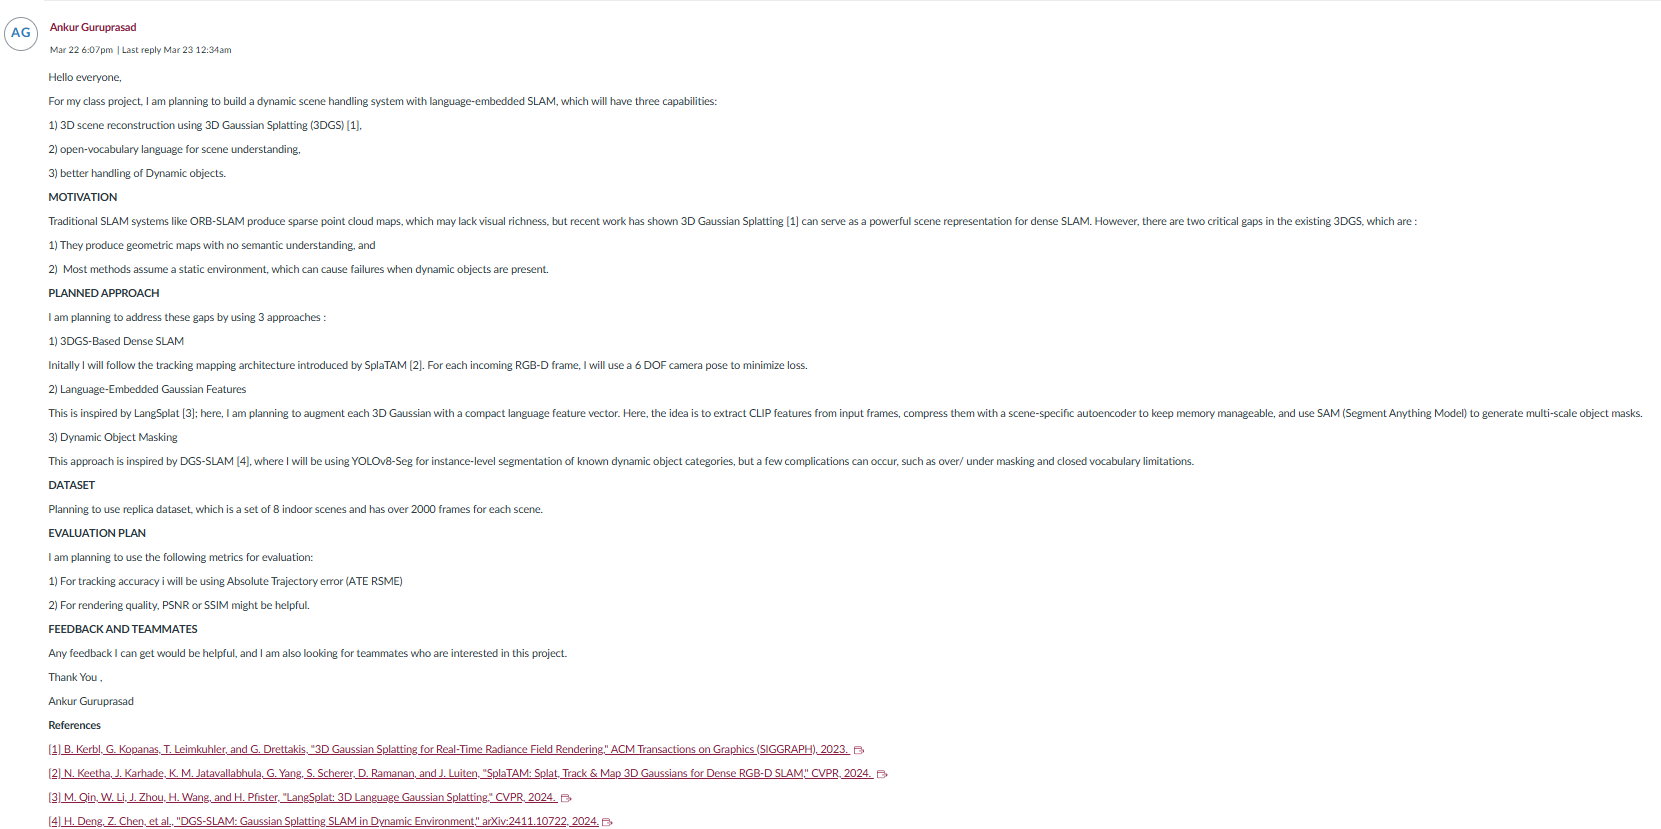
\includegraphics[width=\linewidth]{my_post.png}
    \caption{My discussion post on the Final Project Research Ideas board, describing the DynLang-SLAM project: a dynamic-aware, language-embedded 3D Gaussian Splatting SLAM system.}
    \label{fig:my_post}
\end{figure}

\subsection{Reply 1: Corinne Shankles --- CV FOD Detection}

Corinne proposes using self-supervised methods for Foreign Object Debris (FOD) detection on airport runways, focusing on robustness under fog conditions. I suggested considering real foggy imagery vs.\ synthetic fog simulation, and whether the ViT autoencoder's reconstruction threshold needs recalibration under adverse weather.

\begin{figure}[H]
    \centering
    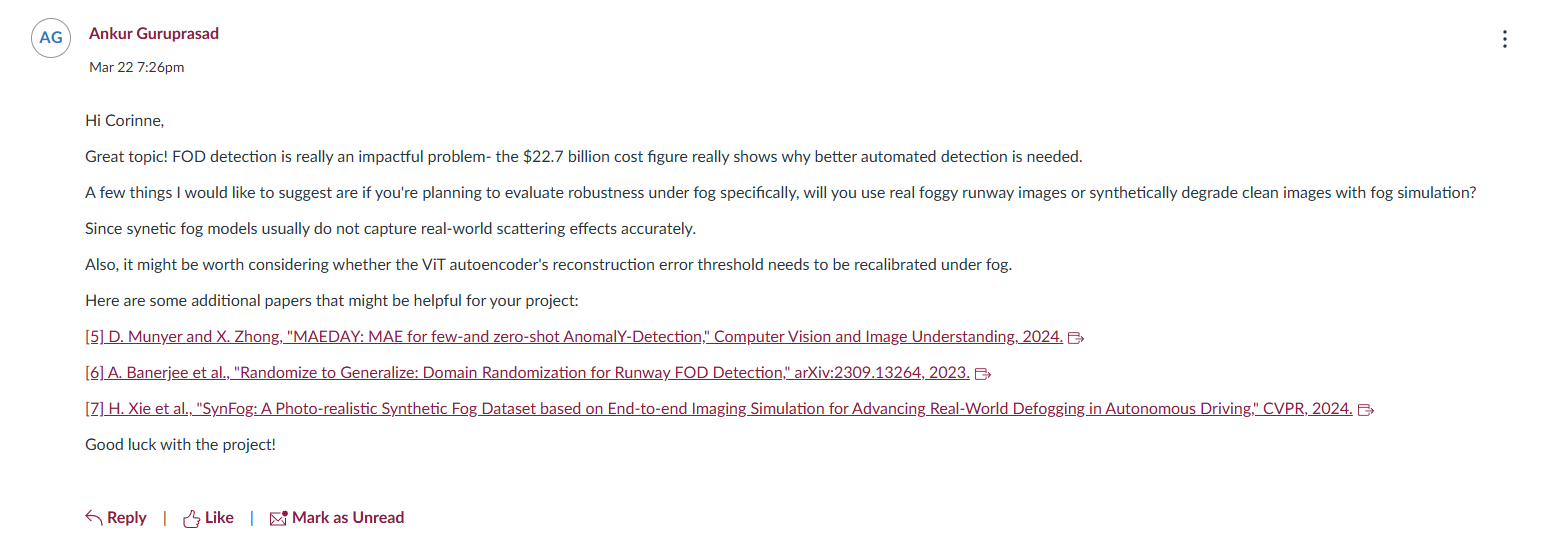
\includegraphics[width=\linewidth]{reply_corinne.png}
    \caption{My reply to Corinne Shankles' post on FOD Detection, with 3 suggested papers on domain randomization, synthetic fog datasets, and anomaly detection.}
    \label{fig:reply_corinne}
\end{figure}

\subsection{Reply 2: Vinith Varghese --- NeRF for Sparse Views}

Vinith proposes implementing NeRF for 3D reconstruction under sparse views and noisy camera poses. I suggested also comparing against 3D Gaussian Splatting (3DGS), which has become the dominant approach since 2023, and recommended using FreeNeRF for regularization under sparse-view settings.

\begin{figure}[H]
    \centering
    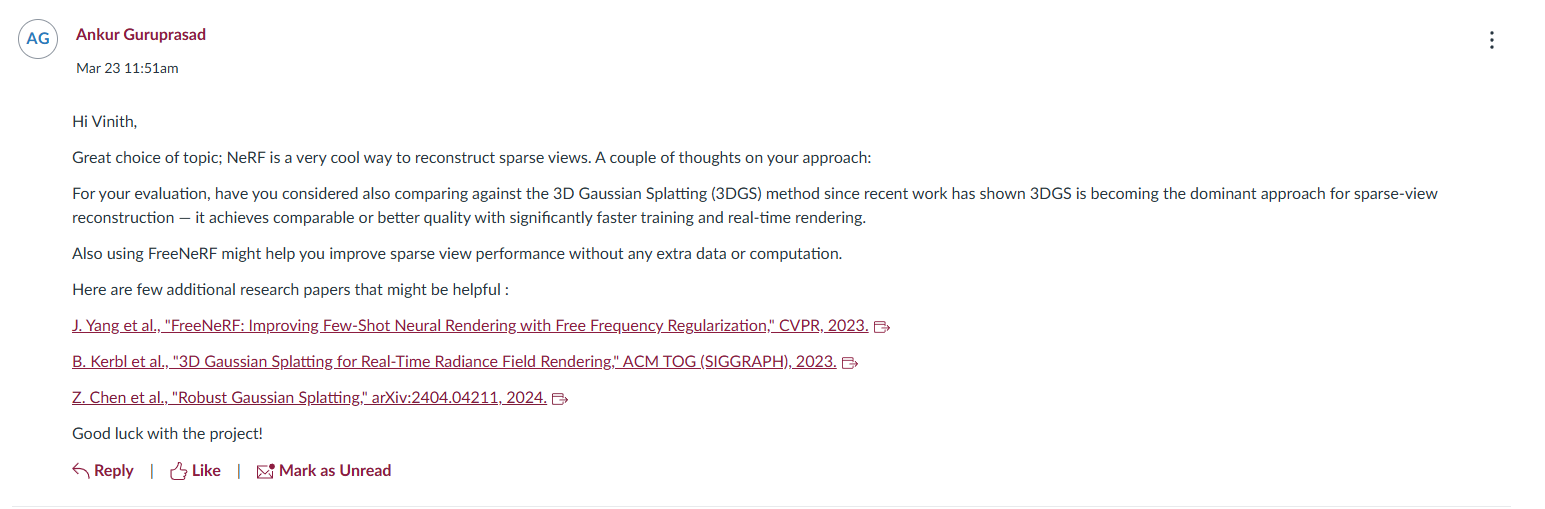
\includegraphics[width=\linewidth]{reply_vinith.png}
    \caption{My reply to Vinith Varghese's post on NeRF sparse-view reconstruction, with 3 suggested papers on 3DGS, FreeNeRF, and robust NeRF methods.}
    \label{fig:reply_vinith}
\end{figure}

\subsection{Reply 3: Rakshit Govind Thota --- Facial Emotion Recognition Failures}

Rakshit proposes studying why facial emotion recognition (FER) models fail under image degradation (blur, noise, occlusion) using Grad-CAM attention analysis. I suggested quantifying the Grad-CAM heatmap shift as a numeric ``attention drift'' metric, and recommended papers on anti-aliased deep convolution networks and collaborative learning transformers for robust FER.

\begin{figure}[H]
    \centering
    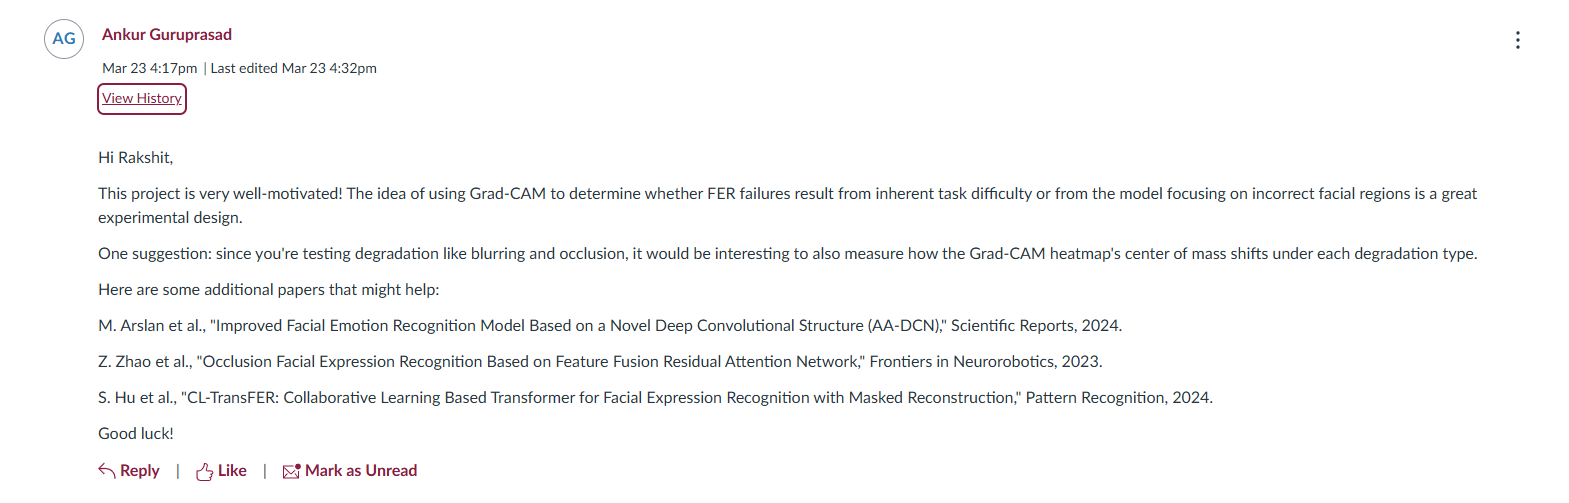
\includegraphics[width=\linewidth]{reply_rakshit.png}
    \caption{My reply to Rakshit Govind Thota's post on facial emotion recognition robustness, with 3 suggested papers on occlusion-aware FER, anti-aliased networks, and masked reconstruction.}
    \label{fig:reply_rakshit}
\end{figure}

% ===================================================================
% References
% ===================================================================
{\small
\begin{thebibliography}{8}

\bibitem{freeman}
W.~T.~Freeman.
\newblock How to do research.
\newblock \url{http://people.csail.mit.edu/billf/www/papers/doresearch.pdf}. MIT CSAIL.

\bibitem{kerbl20233dgs}
B.~Kerbl, G.~Kopanas, T.~Leimk{\"u}hler, and G.~Drettakis.
\newblock 3D Gaussian Splatting for Real-Time Radiance Field Rendering.
\newblock {\em ACM Transactions on Graphics (SIGGRAPH)}, 42(4):1--14, 2023.

\bibitem{keetha2024splatam}
N.~Keetha, J.~Karhade, K.~M.~Jatavallabhula, G.~Yang, S.~Scherer, D.~Ramanan, and J.~Luiten.
\newblock SplaTAM: Splat, Track \& Map 3D Gaussians for Dense RGB-D SLAM.
\newblock In {\em Proc. IEEE/CVF Conf. Computer Vision and Pattern Recognition (CVPR)}, 2024.

\bibitem{qin2024langsplat}
M.~Qin, W.~Li, J.~Zhou, H.~Wang, and H.~Pfister.
\newblock LangSplat: 3D Language Gaussian Splatting.
\newblock In {\em Proc. IEEE/CVF Conf. Computer Vision and Pattern Recognition (CVPR)}, 2024.

\bibitem{deng2024dgsslam}
H.~Deng, Z.~Chen, et~al.
\newblock DGS-SLAM: Gaussian Splatting SLAM in Dynamic Environment.
\newblock {\em arXiv preprint arXiv:2411.10722}, 2024.

\bibitem{matsuki2024monogs}
H.~Matsuki, R.~Murai, P.~H.~J.~Kelly, and A.~J.~Davison.
\newblock Gaussian Splatting SLAM.
\newblock In {\em Proc. IEEE/CVF Conf. Computer Vision and Pattern Recognition (CVPR)}, 2024. Highlight, Best Demo Award.

\bibitem{tosi2025survey}
F.~Tosi, Y.~Zhang, Z.~Gong, E.~Sandstr{\"o}m, S.~Mattoccia, M.~R.~Oswald, and M.~Poggi.
\newblock How NeRFs and 3D Gaussian Splatting are Reshaping SLAM: a Survey.
\newblock {\em arXiv preprint arXiv:2402.13255}, 2024 (updated March 2025).

\bibitem{ding2025survey}
T.~Ding, S.~Gao, Y.~Huang, et~al.
\newblock 3D Gaussian Splatting: Survey, Technologies, Challenges, and Opportunities.
\newblock {\em IEEE Transactions on Circuits and Systems for Video Technology}, 2025.

\end{thebibliography}
}

\end{document}
